\documentclass[11pt]{article}

% ---------------------------------------------------------------------------
%  Plausible Fiction on MeTTaIL --- Requirements & Design
% ---------------------------------------------------------------------------
\usepackage[letterpaper,margin=1in]{geometry}
\usepackage[T1]{fontenc}
\usepackage{lmodern}
\usepackage{microtype}
\usepackage{amsmath,amssymb,mathtools}
\usepackage{stmaryrd}
\usepackage{mathpartir}
\usepackage{booktabs}
\usepackage{array}
\usepackage{enumitem}
\usepackage{titlesec}
\usepackage{fancyhdr}
\usepackage{xcolor}
\usepackage{listings}
\usepackage{tikz}
\usetikzlibrary{automata,positioning,arrows.meta,fit,backgrounds}
\usepackage[hidelinks,colorlinks=true,linkcolor=accent,urlcolor=accent,citecolor=accent]{hyperref}

% ----- palette -------------------------------------------------------------
\definecolor{accent}{HTML}{8A1C1C}      % f1r3 red
\definecolor{ink}{HTML}{1A1A1A}
\definecolor{rule}{HTML}{B0B0B0}
\definecolor{codebg}{HTML}{F6F3EE}
\definecolor{kw}{HTML}{8A1C1C}
\definecolor{kw2}{HTML}{12598A}
\definecolor{cmt}{HTML}{6B7A5A}
\definecolor{str}{HTML}{1F7A4D}
\definecolor{lit}{HTML}{9A6A00}

% ----- headers -------------------------------------------------------------
\pagestyle{fancy}
\fancyhf{}
\renewcommand{\headrulewidth}{0.2pt}
\renewcommand{\footrulewidth}{0pt}
\lhead{\small\textsc{Plausible Fiction on MeTTaIL}}
\rhead{\small\thepage}
\setlength{\headheight}{14pt}
\setlength{\emergencystretch}{1.5em}

\titleformat{\section}{\Large\bfseries\color{accent}}{\thesection}{0.6em}{}
\titleformat{\subsection}{\large\bfseries\color{ink}}{\thesubsection}{0.6em}{}
\titleformat{\subsubsection}{\normalsize\bfseries\color{ink}}{\thesubsubsection}{0.6em}{}

% ----- math shorthands -----------------------------------------------------
\newcommand{\rul}[1]{\ensuremath{\textsc{#1}}}
\newcommand{\Type}{\mathsf{Type}}
\newcommand{\Term}{\mathsf{Term}}
\newcommand{\Pf}{\mathsf{PF}}
\newcommand{\hole}[2]{\ensuremath{?#1\!:\!#2}}
\newcommand{\plug}{\mathbin{\triangleleft}}
\newcommand{\sat}{\models}
\newcommand{\conv}{\equiv}
\newcommand{\subt}{\mathrel{<:}}
\newcommand{\tele}{\Gamma}
\newcommand{\tm}{t}
\newcommand{\Holes}{\ensuremath{\operatorname{holes}}}
\newcommand{\grounded}{\ensuremath{\operatorname{grounded}}}
\DeclareMathOperator{\dom}{dom}

% ----- listings: shared style ----------------------------------------------
\lstdefinestyle{base}{
  backgroundcolor=\color{codebg},
  basicstyle=\ttfamily\footnotesize\color{ink},
  breaklines=true,
  breakatwhitespace=true,
  columns=fullflexible,
  keepspaces=true,
  showstringspaces=false,
  commentstyle=\color{cmt}\itshape,
  stringstyle=\color{str},
  numberstyle=\tiny\color{rule},
  frame=leftline,
  framerule=1.2pt,
  rulecolor=\color{accent},
  xleftmargin=10pt,
  framexleftmargin=8pt,
  aboveskip=8pt,belowskip=8pt,
  literate={->}{{$\rightarrow$}}2 {~>}{{$\;\rightsquigarrow\;$}}2
}

% MeTTaIL language! definitions
\lstdefinelanguage{mettail}{
  morekeywords={language,name,types,literals,terms,equations,rewrites,logic,as,fold,prefix,relation,if,let},
  morekeywords=[2]{Term,HoleId,Ty,Lvl,Tag,Bool,Int,Str,Proc,Name,List,Map,Set,Bag},
  sensitive=true,
  morecomment=[l]{//},
  morestring=[b]",
  keywordstyle=\color{kw}\bfseries,
  keywordstyle=[2]\color{kw2},
}
% Embedded rholang (coordination layer)
\lstdefinelanguage{rho}{
  morekeywords={for,new,in,where,match,contract,Nil,if,else,true,false,and,or,not},
  morekeywords=[2]{plug,holes,grounded,parties,dispatch,monitor,abstract,publish,offer,broker,retire,hide,advertise},
  sensitive=true,
  morecomment=[l]{//},
  morestring=[b]",
  keywordstyle=\color{kw}\bfseries,
  keywordstyle=[2]\color{kw2}\itshape,
}
\lstset{style=base}
\newcommand{\code}[1]{\lstinline[language=rho,basicstyle=\ttfamily\small]|#1|}

% ----- title ---------------------------------------------------------------
\title{\vspace{-2.5em}\color{accent}\textbf{Plausible Fiction on MeTTaIL}\\[0.2em]
  \large\color{ink}\textnormal{A Requirements \& Design Document for a Typed Marketplace of Programmatic Intentions}}
\author{\normalsize F1R3FLY.io \quad$\cdot$\quad in dialogue with D.~Spivak (Topos Institute)}
\date{\normalsize\today \;\; --- \;\; Draft for discussion}

\begin{document}
\maketitle
\thispagestyle{fancy}

\begin{abstract}
\noindent
\emph{Plausible Fiction} (PF) is a marketplace in which a participant publishes a
\emph{programmatic} description of a good or service they want produced --- ``plausible'' because it
is a runnable artifact, ``fiction'' because it contains \emph{holes} that no one party can yet fill.
Following Spivak's original framing, a PF is a term in a dependently typed lambda calculus; a PF with
holes is a \emph{context}. We refine that framing by distinguishing holes that must be filled by
\emph{other agents} in the market from holes that are filled by \emph{ordinary computation}. This
document specifies the system in two layers on top of MeTTaIL (rholang~1.4): (i)~an object language
--- a dependently typed $\lambda$-calculus with typed holes --- given as a MeTTaIL
\lstinline[language=mettail,basicstyle=\ttfamily\small]|language!| definition, whose terms ride on
rho channels; and (ii)~a coordination protocol written in MeTTaIL's built-in embedded rholang that
manages the full PF lifecycle: publish, match, broker, ground, run, monitor, and either promote to a
\emph{template} on success or \emph{retire} (hide or advertise) on failure. Because a PF can branch
on outcomes, its open holes are not a flat list but a \emph{conditional demand tree} (CDT) --- a
finite dependent polynomial fibering the holes owed over the outcomes not yet observed; we make
\lstinline[language=mettail,basicstyle=\ttfamily\small]|holes(.)| return this object and show how the
coordinator arms its immediate frontier while subscribing to its branch edges. We give code
illustrations throughout, a lifecycle state machine, a numbered requirements catalogue, a worked
end-to-end example, and an honest accounting of what is established versus conjectural.
\end{abstract}

\tableofcontents
\vspace{1em}

% ===========================================================================
\section{Purpose and scope}
% ===========================================================================
This document specifies \emph{what} the Plausible Fiction service must do and \emph{how} it maps onto
MeTTaIL, at a level of detail sufficient to begin implementation and to anchor continued design
discussion with the Topos Institute. It is deliberately concrete about the MeTTaIL surface: the
object language is given as a \lstinline[language=mettail,basicstyle=\ttfamily\small]|language!|
specification, and every coordination behaviour is given as embedded rholang. It is deliberately
honest about its open problems (\S\ref{sec:open}): several matching and templating questions are
undecidable in full generality, and the design's central move is to \emph{delegate} those problems to
the market rather than to a solver.

\paragraph{Non-goals.} We do not re-specify rholang itself. MeTTaIL ships an embedded rholang as its
coordination language, and separately offers a language-definition facility (it can even give a
meta-circular account of rho); the latter is what we use to define the object language, and the
former is what we use to coordinate. We treat both as given.

% ===========================================================================
\section{Conceptual model}\label{sec:model}
% ===========================================================================

\subsection{A PF is a typed context}
Fix a dependently typed $\lambda$-calculus with a sort $\Term$ of terms (which, being dependent, also
serves as the sort of types). A \emph{Plausible Fiction} is a $\Term$ that may contain \emph{typed
holes}. Writing $\hole{h}{T}$ for a hole named $h$ with expected type $T$:
\[
  \Pf \;\;::=\;\; \tm \quad\text{where}\quad \tm \text{ ranges over } \Term \text{ with holes } \hole{h}{T}.
\]
A hole is a typed metavariable; a term with holes is exactly a \emph{many-holed context}. The two
defining slogans become precise:
\begin{itemize}[leftmargin=1.4em,itemsep=2pt]
  \item \textbf{Plausible} $=$ the description is a real, type-checkable program fragment, not prose.
  \item \textbf{Fiction} $=$ it has holes; it asserts the \emph{existence} of fillers it does not yet possess.
\end{itemize}

\subsection{Grounding and running}
A PF is \emph{grounded} when it has no \emph{agent} holes (defined next). A grounded PF is a closed
program that can be \emph{run}: every party who contributed a sub-PF performs their part, in the world,
under coordination and monitoring. ``Filling a hole'' is plugging another PF into it; when the last
agent hole is plugged the PF becomes grounded and is eligible to run.

\subsection{Two kinds of hole}\label{sec:twoholes}
This is our refinement of Spivak's model, and it drives the whole lifecycle.
\begin{description}[leftmargin=0pt,style=nextline,itemsep=4pt]
  \item[Agent holes $\hole{h}{T}$.] Filled by \emph{another PF supplied by another participant}.
  These are market demands. They are the only holes that the lifecycle advertises, brokers, and waits
  on. \grounded\ counts \emph{only} agent holes. An agent hole \emph{resolves} in one of two ways,
  which affects only \emph{when}, not \emph{how}, it enters the market (\S\ref{sec:branch}):
  \emph{filler-resolved} (the default --- a market plug supplies it), or \emph{outcome-resolved}
  (an \emph{observation} hole whose value is revealed only by running a step, via attestation).
  \item[Computation holes.] Filled by \emph{standard computation}: $\beta$/$\eta$-reduction,
  normalization, and elaboration of implicit arguments (ordinary metavariables solved by
  unification). These never become market demands; they are discharged by the evaluator/elaborator.
\end{description}
Concretely: a redex such as $(\lambda(x{:}A).b)\,a$ is a computation hole --- it is ``filled'' by
$\beta$. An implicit argument that the elaborator can infer is a computation hole. A slot for ``a
licensed electrician who will wire the venue'' is an agent hole --- no amount of computation produces
the electrician; \emph{another participant} must offer one.

\subsection{Branch-dependent holes and the demand polynomial}\label{sec:branch}
A PF does not merely \emph{have} holes; it \emph{branches}, and which holes are owed can depend on an
outcome that has not landed yet. Spivak's minimal case: Alice books a venue before she knows whether
it will be indoor or outdoor; an outdoor booking owes a rain contingency (a tent), an indoor one must
\emph{not}.
\[
  \texttt{case}\ v\ \texttt{of}\ \{\ \mathsf{Indoor}\ v_{\mathrm{in}} \Rightarrow \mathit{book}\,v_{\mathrm{in}}\,c \mid
     \mathsf{Outdoor}\ v_{\mathrm{out}} \Rightarrow \hole{h_{\mathrm{Tent}}}{\mathsf{Tent}(v_{\mathrm{out}})};\ \mathit{book}\,v_{\mathrm{out}}\,c\,t\ \}
\]
Here $h_{\mathrm{Cater}}$ is owed on \emph{every} branch, while $h_{\mathrm{Tent}}$ is owed
\emph{iff} the venue $v$ resolves $\mathsf{Outdoor}$ --- and its type $\mathsf{Tent}(v_{\mathrm{out}})$
\emph{depends on the outcome's payload}. So the open-hole set is a \emph{function of $v$}, and $v$ is
not yet present when we ask for the holes.

A flat \lstinline[language=mettail,basicstyle=\ttfamily\small]|List of [h, ty]| cannot represent this:
it is wrong on one branch (it either spuriously demands a tent indoors, or omits the tent contingency
outdoors). The two naive escapes both lose something essential:
\begin{description}[leftmargin=0pt,style=nextline,itemsep=2pt]
  \item[Eager (hoist $h_{\mathrm{Tent}}$ up front).] A tent is then demanded, brokered, and waited on
  even for indoor venues --- an obligation that should not exist.
  \item[Lazy (let the venue filler introduce $h_{\mathrm{Tent}}$ on republish).] Operationally fine,
  but then \emph{no PFLam term ever says ``outdoor owes a tent''}: the contingency exists only after a
  filler commits, so the outdoor branch cannot be reasoned about, priced, or checked before grounding.
\end{description}
The branch is already \emph{in the term}, so we take neither escape. We make
\lstinline[language=mettail,basicstyle=\ttfamily\small]|holes(.)| return a \emph{conditional demand
tree} (CDT): a finite tree whose nodes carry a \emph{frontier} of holes armed immediately and in
parallel, and whose edges are \emph{outcomes of a scrutinee} under which a sub-CDT continues. This is a
\emph{dependent polynomial} (an interaction structure): positions are outcome-states, the directions at
a position are the holes owed there. $h_{\mathrm{Cater}}$ lands in the root frontier; $h_{\mathrm{Tent}}$
lives in the fiber over $v=\mathsf{Outdoor}$, with its type binding $v_{\mathrm{out}}$.
Section~\ref{sec:cdt} makes this precise and shows it is computed --- not annotated --- from the term
Alice already wrote.

\subsection{The market is the search procedure}\label{sec:marketsearch}
A subtle but load-bearing observation. ``Types mediate matching'' means a candidate filler $q$ fits a
hole $\hole{h}{T}$ iff $q$ \emph{checks} at type $T$ in the hole's local context. \emph{Checking a
given $q$ against $T$ is decidable} (bidirectional type-checking, assuming normalization).
\emph{Finding} such a $q$ is higher-order search and is undecidable in general. The PF design's answer
is not to run a solver: it is to publish the demand and let other agents \emph{offer} candidates,
which the type guard merely \emph{checks}. The rho market --- forwarders, brokers, offers --- is the
(distributed, human-and-machine, economically incentivized) search procedure; the type system is only
the acceptance test. See \S\ref{sec:open} for the formal consequences.

% ===========================================================================
\section{Architecture}\label{sec:arch}
% ===========================================================================
Three strata (Figure~\ref{fig:arch}):
\begin{enumerate}[leftmargin=1.6em,itemsep=2pt]
  \item \textbf{Object language \texttt{PFLam}} (\S\ref{sec:pflam}): a dependently typed
  $\lambda$-calculus with typed holes, defined with MeTTaIL's
  \lstinline[language=mettail,basicstyle=\ttfamily\small]|language!|. Pure, total operations:
  bidirectional typing, $\Holes(\cdot)$, $\grounded(\cdot)$, and $\plug$.
  \item \textbf{Bridge} (\S\ref{sec:bridge}): a small set of rho-callable predicates/operators ---
  \code{pf |= ty}, \code{grounded(pf)}, \code{plug(pf,h,q)}, \code{holes(pf)} (now returning a CDT),
  and \code{resolve(pf,s)} --- that lift \texttt{PFLam} operations into embedded rholang as
  \texttt{Bool}/payload/\texttt{Name} folds. This is the only place the two layers touch.
  \item \textbf{Coordination} (\S\ref{sec:coord}): embedded rholang protocols implementing the
  lifecycle over per-user channel namespaces.
\end{enumerate}

\begin{figure}[h]
\centering
\resizebox{\textwidth}{!}{%
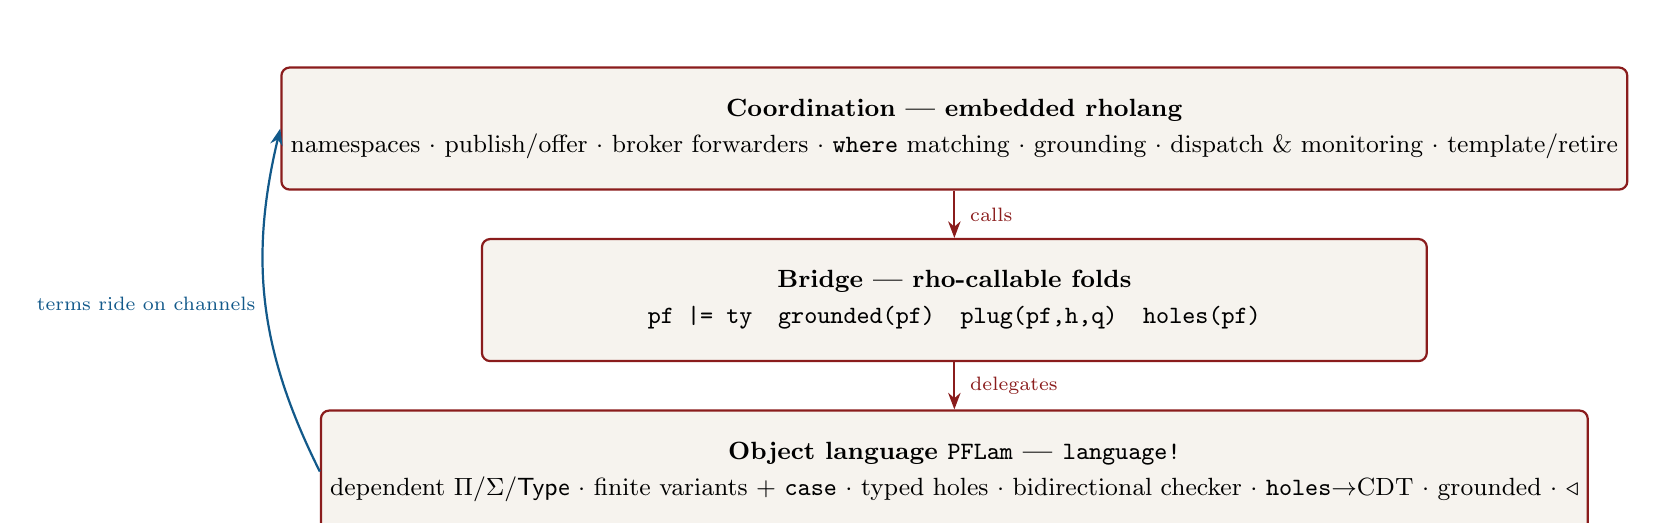
\begin{tikzpicture}[font=\small,node distance=6mm]
  \tikzstyle{layer}=[draw=accent,thick,rounded corners=3pt,fill=codebg,
    minimum width=12cm,minimum height=1.55cm,align=center]
  \node[layer] (coord) {\textbf{Coordination — embedded rholang}\\[2pt]
    namespaces $\cdot$ publish/offer $\cdot$ broker forwarders $\cdot$ \texttt{where} matching
    $\cdot$ grounding $\cdot$ dispatch \& monitoring $\cdot$ template/retire};
  \node[layer,below=of coord] (bridge) {\textbf{Bridge — rho-callable folds}\\[2pt]
    \texttt{pf |= ty}\quad\texttt{grounded(pf)}\quad\texttt{plug(pf,h,q)}\quad\texttt{holes(pf)}};
  \node[layer,below=of bridge] (obj) {\textbf{Object language \texttt{PFLam} — \texttt{language!}}\\[2pt]
    dependent $\Pi/\Sigma/\mathsf{Type}$ $\cdot$ finite variants + \texttt{case} $\cdot$ typed holes
    $\cdot$ bidirectional checker $\cdot$ \texttt{holes}$\to$CDT $\cdot$ $\grounded$ $\cdot$ $\plug$};
  \draw[-{Stealth[length=6pt]},accent,thick] (coord) -- (bridge)
     node[midway,right=2pt,font=\scriptsize]{calls};
  \draw[-{Stealth[length=6pt]},accent,thick] (bridge) -- (obj)
     node[midway,right=2pt,font=\scriptsize]{delegates};
  \draw[-{Stealth[length=6pt]},kw2,thick] (obj.west) to[bend left=20]
     node[midway,left,font=\scriptsize]{terms ride on channels} (coord.west);
\end{tikzpicture}%
}
\caption{The three strata. Object-language terms are payloads carried on rho channels; the bridge is
the sole coupling point.}
\label{fig:arch}
\end{figure}

% ===========================================================================
\section{Object language \texttt{PFLam}}\label{sec:pflam}
% ===========================================================================
We give \texttt{PFLam} as a Pure-Type-System--style dependent calculus with a single sort
$\Term$, a cumulative universe hierarchy, dependent function ($\Pi$) and pair ($\Sigma$) types
(records-as-$\Sigma$ model goods/services), finite dependent \emph{variants} with their eliminator
(\texttt{case}, for outcomes and branching --- the Option~A addition), and the distinguished
\rul{Hole} constructor (with \rul{Obs} for outcome-resolved holes). The surface
syntax is ASCII to match MeTTaIL's existing examples (\lstinline[language=mettail,basicstyle=\ttfamily\small]|lam x.x|, \lstinline[language=mettail,basicstyle=\ttfamily\small]|(f, x)|).

\subsection{Hole interfaces are telescopes}\label{sec:teleholes}
A hole does not float free: it sits under binders and may use the variables in scope at its position.
Its \emph{interface} is therefore a \emph{telescope} $\tele_h$ (the local context) together with an
expected type $T_h$. We encode this by $\Pi$-closing: a hole records the single closed type
$\Pi\tele_h.\,T_h$, and a filler is a closed term of that type, \emph{applied} to the local variables
at the plug site. This is exactly why Spivak's hole-filling reads as application: plugging
\code{alicePF} at hole $h$ with $q$ is, up to bookkeeping, $\mathtt{alicePF}$ with $q$ substituted for
$\hole{h}{\Pi\tele_h.T_h}$ and applied to $\tele_h$. The minimal spec below keeps \rul{Hole} binary
($h$, $T$) with the telescope folded into $T$ via $\Pi$.

\subsection{The \texttt{language!} specification}
\begin{lstlisting}[language=mettail]
language! {
    name: PFLam,

    types {
        Term                       // dependent: terms and types share one sort
        ![String] as HoleId        // agent-hole identifiers (market-visible)
        ![String] as MetaId        // computation-hole / elaboration metavars
        ![String] as Tag           // variant labels (outcome constructors)
        ![u64]    as Lvl           // universe levels
        VariantAlts                // sequence of  (Tag : Term)   alternatives
        CaseBranch                 // one  (Tag x => body)  arm
        CaseBranches               // sequence of CaseBranch
    },

    terms {
        // ---- core dependent calculus -------------------------------------
        Univ . l:Lvl                      |- "Type" l            : Term;
        Var  . x:Term                     |- x                   : Term;  // bound via HOAS below

        Pi   . dom:Term, ^x.cod:[Term -> Term]
             |- "Pi" "(" x ":" dom ")" "." cod                   : Term;
        Lam  . dom:Term, ^x.body:[Term -> Term]
             |- "lam" "(" x ":" dom ")" "." body                 : Term;
        App  . fun:Term, arg:Term         |- "(" fun " " arg ")" : Term;

        // dependent records model goods/services as Sigma-bundles
        Sig  . fst:Term, ^x.snd:[Term -> Term]
             |- "Sig" "(" x ":" fst ")" "." snd                  : Term;
        Pair . a:Term, b:Term             |- "<" a "," b ">"     : Term;
        Fst  . p:Term                     |- "fst" p             : Term;
        Snd  . p:Term                     |- "snd" p             : Term;

        // ---- finite (dependent) variants: model outcomes / branching -----
        // A finite labelled sum  < l_1 : A_1 | ... | l_n : A_n >  (Spivak's O_venue).
        Variant . alts:VariantAlts        |- "<" alts ">"        : Term;
        Alt     . lbl:Tag, ty:Term        |- lbl ":" ty          : VariantAlts;  // seq-folded
        Inj     . lbl:Tag, val:Term       |- "inj" lbl val       : Term;
        // Dependent eliminator: motive mot, one arm per label; the arm binds the payload.
        Case    . scrut:Term, mot:Term, brs:CaseBranches
                |- "case" scrut "of" "{" brs "}"                 : Term;
        CaseBr  . lbl:Tag, ^x.body:[Term -> Term]
                |- lbl " " x "=>" body                           : CaseBranch;

        // ---- THE distinguishing constructors -----------------------------
        // Agent hole (filler-resolved): supplied by another participant's PF.
        // ty is the Pi-closed interface  Pi Gamma_h . T_h  (see sec. 4.1).
        Hole . h:HoleId, ty:Term          |- "?" h ":" ty        : Term;

        // Observation hole (outcome-resolved): an agent hole whose value is
        // revealed by RUNNING a step (attestation), not by a market plug. It is
        // a legitimate case-scrutinee and a CDT branch point (sec. 4.4, 6.x).
        Obs  . h:HoleId, ty:Term          |- "observe" h ":" ty  : Term;

        // Computation hole: an elaboration metavariable, solved by unification.
        // NEVER advertised to the market; discharged by the elaborator.
        Meta . m:MetaId, ty:Term          |- "%" m ":" ty        : Term;

        // ---- pure operations exposed to the bridge -----------------------
        // grounded(p): the REALIZED path carries no agent holes. Reduction now
        // includes case-reduction (CaseRw), so once a scrutinee hole resolves
        // its branch is taken and only that branch's holes remain (sec. 4.4).
        Grounded . p:Term  |- "grounded" "(" p ")" : Term ![{
            crate::pflam::no_agent_holes(&p)        // -> Term::BoolLit(_)
        }] fold;

        // holes(p): the open agent demands as a CONDITIONAL DEMAND TREE (sec 4.4)
        // -- a finite dependent polynomial: a now-frontier of holes armed in
        // parallel, plus outcome-indexed edges over unresolved scrutinees.
        // NOT a flat list: the owed-set is a function of outcomes not yet seen.
        HolesOf  . p:Term  |- "holes" "(" p ")"    : Term ![{
            crate::pflam::demand_tree(&p)           // -> CDT (see grammar, sec 4.4)
        }] fold;

        // plug(p, h, q): fill agent hole h in p with filler q (capture-avoiding;
        // q is the Pi-closed filler, re-applied to the local telescope).
        Plug . p:Term, h:HoleId, q:Term
             |- "plug" "(" p "," h "," q ")"        : Term ![{
            crate::pflam::plug_hole(&p, &h, &q)
        }] fold;
    },

    equations {
        // beta / eta / projection are CONVERSION (the equational theory used by
        // type conversion and by the matching test |=).
        Beta . |- ( (lam (x : A) . b) a ) = (subst b x a) ;
        Eta  . |- (lam (x : A) . (f x)) = f ;          // x not free in f
        SigB1 . |- (fst < a , b >) = a ;
        SigB2 . |- (snd < a , b >) = b ;
        // variant beta: case of a known injection selects and substitutes its arm.
        CaseB . |- (case (inj l a) mot { ... ; l x => body ; ... }) = (subst body x a) ;
    },

    rewrites {
        // directed reduction = "filling computation holes by standard computation"
        BetaRw . |- ( (lam (x : A) . b) a ) ~> (subst b x a) ;
        Fst1   . |- (fst < a , b >) ~> a ;
        Snd1   . |- (snd < a , b >) ~> b ;
        // CASE on a KNOWN injection reduces (computation). On a NEUTRAL scrutinee
        // -- one stuck on an unresolved Hole/Obs -- it does NOT reduce: it is a
        // branch point of the demand tree (sec. 4.4).
        CaseRw . |- (case (inj l a) mot brs) ~> (selectArm brs l a) ;
        // plug reduces structurally once its filler is present; if it resolves a
        // scrutinee, the enclosing CaseRw then fires, realizing a branch.
        PlugRw . |- (plug p h q) ~> (subst_hole p h q) ;
        // congruences (elided): AppCongL/R, PiCong, LamCong, SigCong, PairCong,
        //                       CaseCongScrut, CaseCongArm, ...
    },

    logic {
        // Bidirectional typing as an ascent relation (sketch, sec. 4.3).
        // check(ctx, term, ty)  and  synth(ctx, term, ty).
        // matching test:  models(q, ty)  iff  exists A. synth([], q, A), sub(A, ty).
        relation check(Ctx, Term, Term);
        relation synth(Ctx, Term, Term);
        relation sub(Term, Term);                 // conversion + universe cumulativity
        relation models(Term, Term);
        models(q, ty) <-- synth(ctx0(), q, a), sub(a, ty);
    },
}
\end{lstlisting}

\subsection{Bidirectional typing and the matching relation}\label{sec:typing}
The equational theory ($\beta\eta$, projections) is \emph{conversion}, written $\conv$. Subtyping
$\subt$ is conversion plus universe cumulativity (and, optionally, width/depth subtyping on
$\Sigma$-records, which is exactly what lets a richer offer satisfy a leaner demand). The judgments
are the usual bidirectional pair; the rules that matter for matching are:

\begin{mathpar}
\inferrule[Hole-Synth]{ }{\tele \vdash \hole{h}{T} \Rightarrow T}
\and
\inferrule[Sub]{\tele \vdash \tm \Rightarrow A \\ A \subt B}{\tele \vdash \tm \Leftarrow B}
\and
\inferrule[Pi]{\tele \vdash A \Leftarrow \Type_i \\ \tele, x{:}A \vdash B \Leftarrow \Type_i}
          {\tele \vdash \Pi(x{:}A).B \Rightarrow \Type_i}
\and
\inferrule[Lam]{\tele, x{:}A \vdash b \Leftarrow B}
          {\tele \vdash \lambda(x{:}A).b \Leftarrow \Pi(x{:}A).B}
\and
\inferrule[App]{\tele \vdash f \Rightarrow \Pi(x{:}A).B \\ \tele \vdash a \Leftarrow A}
          {\tele \vdash f\,a \Rightarrow B[a/x]}
\end{mathpar}

\noindent
\textbf{Matching.} A candidate filler $q$ \emph{satisfies} a hole $\hole{h}{T}$ --- written
$q \sat T$ --- iff $\tele_h \vdash q \Leftarrow T$, equivalently (\rul{Sub}) iff $q$ synthesizes some
$A$ with $A \subt T$. This is the predicate the rho \code{where} guard evaluates. It is decidable on
the chosen normalizing fragment; the search for $q$ is \emph{not} performed here (\S\ref{sec:marketsearch}).

\paragraph{Plugging, precisely.} For $q \sat T_h$,
\[
  p \plug_h q \;\;:=\;\; \mathtt{subst\_hole}(p, h, q),
\]
the capture-avoiding replacement of every $\hole{h}{T_h}$ in $p$ by $q$ (with $q$ applied to the local
telescope $\tele_h$ per \S\ref{sec:teleholes}). \emph{Crucially, $q$ may itself contain agent holes.}
On the \emph{flat} fragment (no branching) this gives the hole-set recurrence
\(
  \Holes(p \plug_h q) = (\Holes(p)\setminus\{h\}) \cup \Holes(q),
\)
the recursive engine of the marketplace: filling a hole can introduce new holes, deferred to new
participants. With branching this becomes a splice on the demand \emph{tree} rather than the set, and
if $h$ was a \emph{scrutinee} its plug fires \rul{CaseRw}, realizing a branch and pruning the others
(\S\ref{sec:cdt}). $\grounded(p)$ holds iff the demand tree of the realized path is empty.

\subsection{The demand polynomial: \texttt{holes(\(\cdot\))} as a CDT}\label{sec:cdt}
This section makes \S\ref{sec:branch} precise: what
\lstinline[language=mettail,basicstyle=\ttfamily\small]|holes(p)| returns for an un-grounded,
\emph{branching} term, and why it is computed rather than annotated.

\paragraph{The object.} A \emph{conditional demand tree} is
\[
  \mathrm{CDT} \;::=\; \big\langle\, \mathsf{now}:\mathsf{Frontier},\ \ \mathsf{wait}:\overline{\mathsf{Edge}} \,\big\rangle,
  \qquad
  \mathsf{Frontier} \;::=\; \overline{(h:T)},
\]
\[
  \mathsf{Edge} \;::=\; \mathsf{on}(s)\,\{\, \overline{\kappa_i\,x_i \Rightarrow \mathrm{CDT}_i} \,\},
\]
where $\mathsf{now}$ is a finite set of holes armed \emph{immediately and in parallel}; each
$\mathsf{Edge}$ is a \emph{subscription} on a scrutinee $s$ (a neutral term stuck on an unresolved
$\rul{Hole}$ or $\rul{Obs}$), with one continuation per constructor $\kappa_i$ of $s$'s variant type,
binding the outcome payload $x_i$ (so $\mathrm{CDT}_i$ and its hole-types may mention $x_i$). This is
exactly a finite \emph{dependent polynomial} / interaction structure: positions are outcome-states,
the directions at a position are the holes owed there, the responses are the outcomes. $\mathsf{now}$
and $\mathsf{wait}$ at one node are concurrent --- arm every $\mathsf{now}$ demand \emph{and}
subscribe to every edge at once.

\paragraph{Computing it (and why it halts).} \lstinline[language=mettail,basicstyle=\ttfamily\small]|holes(p)| is a two-step fold:
\begin{enumerate}[leftmargin=1.6em,itemsep=2pt]
  \item \emph{Symbolic normalization.} Reduce $p$ with agent holes held \emph{opaque} (neutral).
  Strong normalization of grounded \texttt{PFLam} --- preserved by finite variants
  (\S\ref{sec:open}) --- guarantees this terminates, yielding a \emph{demand normal form}: a tree of
  $\rul{Case}$s on neutral scrutinees with hole-demands at the leaves.
  \item \emph{Extraction + hoist.} Read it structurally: a demand $\hole{h}{T}$ not under any
  unresolved $\rul{Case}$ joins $\mathsf{now}$; a $\rul{Case}$ on neutral $s$ yields an
  $\mathsf{on}(s)\{\dots\}$ edge, recursively. Then iterate the \emph{distributive law}
  \[
    \mathsf{on}(s)\{\, \kappa_i \Rightarrow (\,\mathrm{owe}(h{:}T)\parallel e_i\,) \,\}_i
    \quad\equiv\quad
    \mathrm{owe}(h{:}T)\ \parallel\ \mathsf{on}(s)\{\, \kappa_i \Rightarrow e_i \,\}_i
    \qquad
    \text{(if } s,x_i \notin \mathrm{fv}(T)\text{)}
  \]
  to a fixpoint: a demand owed on \emph{every} branch, and whose type does not mention the outcome,
  hoists to the parent frontier.
\end{enumerate}
The side condition does the real work. It hoists $h_{\mathrm{Cater}}$ (owed on both branches, type
outcome-independent) all the way to the root $\mathsf{now}$, while $h_{\mathrm{Tent}}$ \emph{cannot}
hoist past $\mathsf{on}(v)$ because its type $\mathsf{Tent}(v_{\mathrm{out}})$ binds the outcome. The
\emph{type dependency} --- decidably checked --- is precisely what fibers the demand. The fixpoint is
canonical: each hole sits at the highest node at which its type is well-formed, i.e.\ it is armed as
early as its dependencies permit and no earlier.

\paragraph{Spivak's example.} For \code{alicePF} (\S\ref{sec:example}),
\[
  \Holes(\mathtt{alicePF}) =
  \Big\langle\, \mathsf{now}=\{\,h_{\mathrm{Venue}}:\!O_{\mathrm{venue}},\ h_{\mathrm{Cater}}:\!\mathsf{Catering}\,\},\ \,
  \mathsf{wait}=\big[\,\mathsf{on}(h_{\mathrm{Venue}})\,\mathcal{B}\,\big] \,\Big\rangle,
\]
\[
  \mathcal{B} = \{\ \mathsf{Indoor}\;v_{\mathrm{in}} \Rightarrow \langle\varnothing,[\,]\rangle,
       \quad \mathsf{Outdoor}\;v_{\mathrm{out}} \Rightarrow \langle\{\,h_{\mathrm{Tent}}:\mathsf{Tent}(v_{\mathrm{out}})\,\},[\,]\rangle\ \}.
\]
$h_{\mathrm{Cater}}$ and $h_{\mathrm{Venue}}$ are armed now, in parallel; $h_{\mathrm{Tent}}$ is owed
\emph{iff} $h_{\mathrm{Venue}}$ resolves $\mathsf{Outdoor}$, with a type that depends on which outdoor
venue (Figure~\ref{fig:cdt}).

\begin{figure}[h]
\centering
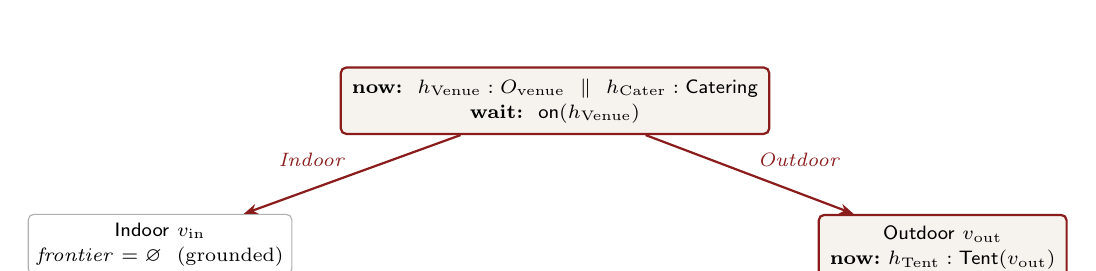
\begin{tikzpicture}[font=\scriptsize,>={Stealth[length=5pt]},
   nd/.style={draw=accent,thick,rounded corners=2pt,fill=codebg,align=center,inner sep=4pt},
   lf/.style={draw=rule,rounded corners=2pt,fill=white,align=center,inner sep=3pt}]
  \node[nd] (root) {\textbf{now:}\ \ $h_{\mathrm{Venue}}:O_{\mathrm{venue}}$\ \ $\parallel$\ \ $h_{\mathrm{Cater}}:\mathsf{Catering}$\\[1pt]
     \textbf{wait:}\ \ $\mathsf{on}(h_{\mathrm{Venue}})$};
  \node[lf,below left=10mm and 6mm of root] (ind) {$\mathsf{Indoor}\ v_{\mathrm{in}}$\\[1pt]\emph{frontier} $=\varnothing$\ \ (grounded)};
  \node[nd,below right=10mm and 6mm of root] (out) {$\mathsf{Outdoor}\ v_{\mathrm{out}}$\\[1pt]\textbf{now:}\ $h_{\mathrm{Tent}}:\mathsf{Tent}(v_{\mathrm{out}})$};
  \draw[->,accent,thick] (root) -- (ind) node[midway,above left=-1pt,font=\scriptsize\itshape]{Indoor};
  \draw[->,accent,thick] (root) -- (out) node[midway,above right=-1pt,font=\scriptsize\itshape]{Outdoor};
\end{tikzpicture}
\caption{The CDT of \code{alicePF}. The root frontier ($h_{\mathrm{Cater}}$, $h_{\mathrm{Venue}}$) is
armed at publish; the $h_{\mathrm{Tent}}$ demand exists in the term \emph{now} (so the Outdoor branch
can be priced and checked) but is \emph{armed} only when $h_{\mathrm{Venue}}$ resolves Outdoor.}
\label{fig:cdt}
\end{figure}

\noindent
This is the third way out of the eager/lazy dilemma (\S\ref{sec:branch}): the contingency is
\emph{stated} in the term (so reasoning, pricing, and checking happen pre-grounding, recovering
``lazy''\,'s loss), yet \emph{armed} only on the realizing outcome (so indoor venues carry no spurious
tent obligation, avoiding ``eager''\,'s loss). When does a scrutinee resolve? If $s$ is a
filler-resolved \rul{Hole} whose type is a variant, plugging the filler reduces the $\rul{Case}$ at
\emph{ground time} and the coordinator arms the sub-CDT during matching. If $s$ is an \rul{Obs} hole,
the branch fires at \emph{run time} on attestation. The CDT shape is identical; only the stage differs,
and it is read off the hole's kind.

% ===========================================================================
\section{The bridge}\label{sec:bridge}
% ===========================================================================
MeTTaIL lets a defined language's terms be sent on rho channels. The coordination layer therefore
carries \texttt{PFLam} terms as payloads and needs five host predicates/operators, each a rho fold
that delegates to \texttt{PFLam}. We extend the embedded coordination language with:

\begin{lstlisting}[language=mettail]
// Bridge operators (rho-level folds delegating to PFLam). Surface syntax in
// the coordination layer; pf, ty, q are embedded PFLam terms carried as payload.

Models   . pf:Proc, ty:Proc  |- pf "|=" ty            : Proc ![{
    // decidable bidirectional check: PFLam.check(ctx_h, pf, ty)
    bool_proc(crate::pflam::models(&pf, &ty))
}] fold;

GroundedP. pf:Proc            |- "grounded" "(" pf ")" : Proc ![{
    bool_proc(crate::pflam::no_agent_holes(&pf))
}] fold;

PlugP    . pf:Proc, h:Proc, q:Proc
         |- "plug" "(" pf "," h "," q ")"              : Proc ![{
    crate::pflam::plug_hole_payload(&pf, &h, &q)       // -> embedded PFLam term
}] fold;

// holes(pf) now returns a CONDITIONAL DEMAND TREE (sec. 4.4), not a list:
//   < now: [[h,ty]...], wait: [ on(s){ [kappa, contFn] ... } ... ] >
// where each cont is the sub-CDT as a function of the bound outcome payload.
HolesP   . pf:Proc            |- "holes" "(" pf ")"    : Proc ![{
    crate::pflam::demand_tree_payload(&pf)             // -> CDT payload
}] fold;

// resolve(pf, s): the channel on which scrutinee s's outcome arrives. For a
// filler-resolved Hole it is derived from the plug (the filler's variant tag +
// payload); for an Obs hole it is the run-time attestation channel. Lets the
// coordinator SUBSCRIBE to a branch edge and continue with the right sub-CDT.
Resolve  . pf:Proc, s:Proc    |- "resolve" "(" pf "," s ")" : Proc ![{
    crate::pflam::resolve_channel(&pf, &s)             // -> Name (a rho channel)
}] fold;
\end{lstlisting}

\noindent
With these in scope, the matching guard Spivak's framing asks for is literally a rholang
\code{where} clause: \code{where pf |= ty}. Everything in \S\ref{sec:coord} is ordinary embedded
rholang plus these operators: \code{now}-frontier holes become guarded demands, and \code{wait}-edges
become \code{resolve}-subscriptions.

% ===========================================================================
\section{Coordination protocol (embedded rholang)}\label{sec:coord}
% ===========================================================================

\subsection{Namespaces and channel conventions}\label{sec:ns}
To each user (say \code{alice}) we associate a namespace of channels, addressed by \emph{quoting}
structured names. We write channels as quoted lists; e.g.\ \code{@[alice, "demand", h]} is the demand
channel for hole \code{h} of one of Alice's PFs. Conventions:

\begin{center}\small
\renewcommand{\arraystretch}{1.25}
\begin{tabular}{@{}>{\ttfamily}l l@{}}
\toprule
\normalfont\textbf{Channel} & \textbf{Role} \\
\midrule
@[u, "pf", pfId]            & canonical store of user \textit{u}'s PF \textit{pfId} (latest term) \\
@[u, "demand", pfId, h]    & open agent hole \textit{h}: candidates are offered here \\
@[u, "resolve", pfId, s]   & outcome of scrutinee \textit{s} (filler tag at ground time, or attestation) \\
@[u, "supply"]             & \textit{u} publishes grounded/partial PFs it offers to others \\
@[u, "prov", pfId]         & provenance map: hole $\mapsto$ (party, fillerId) \\
@[u, "ground", pfId]       & fires once \textit{pfId} becomes grounded \\
@[u, "run", pfId]          & execution controller for a grounded \textit{pfId} \\
@[u, "step", pfId, k]      & attestation channel for execution step \textit{k} \\
@["mkt", "templates"]      & public registry of successful PFs (templates) \\
@["mkt", "caveats"]        & public registry of advertised failures (anti-templates) \\
\bottomrule
\end{tabular}
\end{center}

\subsection{Publish: Draft $\to$ Published}\label{sec:publish}
Publishing stores the PF and walks its \emph{conditional demand tree} (\S\ref{sec:cdt}): it arms one
persistent, type-guarded demand for every hole in the current \code{now}-frontier, and \emph{subscribes}
to every \code{wait}-edge so that a sub-CDT is armed only when its scrutinee resolves. Each demand is
the generalization of Spivak's
\code{for( pf <- aliceChan where pf |= type ){ aliceChan!( (alicePF pf) ) }}; the subscription is the
new ingredient that makes branch-dependent holes (the tent) behave correctly.

\begin{lstlisting}[language=rho]
// publish(u, pfId, pf): store, then arm the CDT of pf.
new publish, armCDT in {
  contract publish(@u, @pfId, @pf) = {
    @[u, "pf", pfId]!!( pf )                          // canonical store (persistent)
    | for( @cdt <- holes(pf) ) { armCDT!( u, pfId, cdt ) }
  }
  |
  // armCDT walks one CDT node: arm every now-hole in PARALLEL, and subscribe to
  // every wait-edge so sub-CDTs are armed only on the realizing outcome.
  contract armCDT(@u, @pfId, @cdt) = {
    match cdt {
      < now: [], wait: [] >      => @[u, "ground", pfId]!( pf )   // realized path empty
      < now: ns,  wait: ws >     => {
        // (1) frontier: one guarded persistent demand per now-hole, all concurrent
        for( @[h, ty] <- ns ) { armDemand!( u, pfId, h, ty ) }
        // (2) edges: subscribe to each scrutinee; arm the matching sub-CDT on resolve
        | for( @on(s, branches) <- ws ) {
            for( @out <- resolve(pf, s) ) {            // outcome arrives (ground- or run-time)
              match out {
                // pick the branch for the realized constructor, binding its payload x,
                // and arm that sub-CDT (its hole-types may mention x).
                @[kappa, x] => armCDT!( u, pfId, select(branches, kappa, x) )
              }
            }
          }
      }
    }
  }
  |
  // one guarded, persistent demand for hole h with expected type ty
  contract armDemand(@u, @pfId, @h, @ty) = {
    for( @cand <= @[u, "demand", pfId, h] where cand |= ty ) {   // type mediates matching
      for( @pf <- @[u, "pf", pfId] ) {                          // read current term
        new pf2 in {
          pf2!( plug(pf, h, cand) ) |                            // fill the hole
          for( @next <- pf2 ) {
            recordProvenance!( u, pfId, h, cand ) |
            // if h was a scrutinee, plug fired CaseRw: the branch is now realized,
            // so re-deriving holes(next) yields the correct residual CDT.
            republish!( u, pfId, next )
          }
        }
      }
    }
  }
}
\end{lstlisting}

\noindent
Notes. (i)~The frontier holes are armed \emph{concurrently} --- \code{hCater} and \code{hVenue} race
freely; neither waits on the other. (ii)~A \code{wait}-edge arms nothing until \code{resolve(pf,s)}
delivers an outcome, so the \emph{indoor} path never arms \code{hTent}. (iii)~\code{resolve} unifies
the two stages: for a filler-resolved scrutinee it fires when the plug commits a variant (ground
time); for an \code{Obs} scrutinee it fires on attestation (run time). (iv)~\code{republish} re-enters
\code{publish}, re-deriving the CDT of the new term --- this is where a filler's own holes, and any
branch just realized, become the next frontier.

\subsection{Offer: supply side}\label{sec:offer}
Bob offers a PF by sending it where a broker (or Alice directly) can pick it up. In the minimal form
this is Spivak's \code{bobChan!( bobPF )}:
\begin{lstlisting}[language=rho]
// Bob advertises a (possibly still-holed) PF he is willing to provide.
@[bob, "supply"]!!( bobPF )
\end{lstlisting}

\subsection{Broker: forwarders with optional type filtering}\label{sec:broker}
A broker connects supply to demand by creating forwarders. The bare forwarder is Spivak's
\code{for( pf <- bobChan ){ aliceChan!( pf ) }}; we add the type guard so the broker only forwards
plausibly-matching candidates and does not spam Alice's demand:
\begin{lstlisting}[language=rho]
// broker(bob -> alice@(pfId,h:ty)): forward Bob's supply to Alice's demand,
// pre-filtered by the hole type so only viable candidates flow.
contract broker(@bob, @alice, @pfId, @h, @ty) = {
  for( @cand <= @[bob, "supply"] where cand |= ty ) {
    @[alice, "demand", pfId, h]!( cand )      // Alice's guarded demand re-checks and plugs
  }
}
\end{lstlisting}

\noindent
The double check (broker filters, demand re-checks) is intentional: the broker's filter is an
optimization; the demand's guard is the authority. Brokers may be matchmakers, reputation services, or
auctions; none of them can cause an ill-typed plug, because the plug only happens behind Alice's
guard.

\subsection{Partial grounding and recursion}
Each successful plug transforms the demand tree, not merely a flat set: \code{republish} re-derives
\code{holes(next)}, which re-arms the residual \code{now}-frontier (old minus $h$, plus $q$'s own
frontier) and re-subscribes to the residual edges. If $h$ was a scrutinee, its plug realized a branch,
so the residual CDT is the corresponding fiber --- the untaken branches and their holes are gone. The
market thus explores a tree of sub-PFs of unbounded depth, each node owned by whichever participant
supplied it. Termination of \emph{a particular} PF is exactly: every realized path eventually reaches
grounded fillers --- a liveness property of the market, not a theorem (\S\ref{sec:open}).

\subsection{Grounding detection: $\to$ Grounded}
Grounding is now \emph{path-realized}, not set-empty. As branches resolve, \rul{CaseRw} prunes the
untaken arms, and \code{holes(pf)} of the residual term shrinks toward
\code{< now: [], wait: [] >}. When \code{armCDT} reaches that node --- the realized path owes nothing
and waits on nothing --- it emits on \code{@[u,"ground",pfId]}. That event is the precondition for
execution. (A PF with an unresolved \code{Obs} edge is \emph{not} grounded: it still waits on a
run-time outcome, so its tail is executed under monitoring rather than dispatched up front ---
\S\ref{sec:exec}.)

\subsection{Execution: Grounded $\to$ Running}\label{sec:exec}
Running a grounded PF means: walk its plan, dispatch each leaf obligation to the party who supplied it
(read from provenance), and collect attestations. Because the obligations are discharged \emph{in the
world}, attestations are signed acknowledgements on per-step channels (oracles); rho coordinates and
records, it does not perform the physical work.

\begin{lstlisting}[language=rho]
// run(u, pfId): dispatch obligations and start the monitor.
contract run(@u, @pfId) = {
  for( @pf <- @[u, "ground", pfId] ; @prov <- @[u, "prov", pfId] ) {
    new steps in {
      steps!( plan(pf, prov) ) |                 // ordered/partially-ordered obligations
      for( @plan <- steps ) {
        dispatch!( u, pfId, plan ) |             // notify each party of its step
        monitor!( u, pfId, plan, 0 )             // begin monitoring at step 0
      }
    }
  }
}

// dispatch: tell each contributing party what to do, on their own channel.
contract dispatch(@u, @pfId, @plan) = {
  for( @[party, k, obligation] <= @plan ) {      // stream the plan's leaves
    @[party, "todo", pfId, k]!( obligation )     // party performs, then attests on step k
  }
}
\end{lstlisting}

\subsection{Monitoring, barriers, and coordination}\label{sec:monitor}
The monitor advances only on positive attestation, joins steps that must complete together (a
\emph{barrier} via multi-receive \code{&}), and routes timeouts/negative acks to failure.
\begin{lstlisting}[language=rho]
// monitor advances step-by-step; a barrier step waits on several attestations at once.
contract monitor(@u, @pfId, @plan, @k) = {
  for( @stepK <- stepAt(plan, k) ) {
    match stepK {
      // ordinary step: one attestation
      [party, k, _] =>
        for( @ack <- @[u, "step", pfId, k] where ack == "ok" ) {
          advance!( u, pfId, plan, k )
        }
      // barrier step: all listed parties must attest before advancing
      [barrier, ks] =>
        for( @a <- @[u,"step",pfId, nth(ks,0)] where a == "ok"
           & @b <- @[u,"step",pfId, nth(ks,1)] where b == "ok" ) {     // ... & ... per ks
          advance!( u, pfId, plan, k )
        }
    }
  }
  // failure routing (timeout or negative attestation) handled in parallel:
  | for( @ack <- @[u, "step", pfId, k] where ack != "ok" ) {
      fail!( u, pfId, pfId )                      // -> retirement (sec. 6.11)
    }
}

// advance: last step -> success; otherwise continue.
contract advance(@u, @pfId, @plan, @k) = {
  match isLast(plan, k) {
    true  => succeed!( u, pfId )
    false => monitor!( u, pfId, plan, k + 1 )
  }
}
\end{lstlisting}

\paragraph{On timeouts.} Pure rho has no clock; ``timeout'' is supplied by an external timer oracle
that posts a non-\code{"ok"} attestation on the step channel after a deadline. The monitor treats it
uniformly as a failed step.

\subsection{Success $\to$ Template}\label{sec:template}
If every step attests \code{"ok"}, the PF \emph{and its sub-PFs} become reusable templates. Templating
is \emph{re-abstraction}: take the grounded composite and reintroduce holes at the positions that were
filled (per provenance), yielding a parametric PF that can be re-grounded with different fillers later.
The principled version of ``reintroduce holes at the filled positions'' is anti-unification (least
general generalization) over the filled subterms (\S\ref{sec:open}).
\begin{lstlisting}[language=rho]
contract succeed(@u, @pfId) = {
  for( @pf <- @[u, "pf", pfId] ; @prov <- @[u, "prov", pfId] ) {
    new tmpl in {
      tmpl!( abstract(pf, prov) ) |               // re-introduce holes at filled positions
      for( @t <- tmpl ) {
        @["mkt", "templates"]!!( [u, pfId, t] )   // publish reusable template
        | @[u, "supply"]!!( t )                    // u can now offer the pattern to others
      }
    }
  }
}
\end{lstlisting}

\subsection{Failure $\to$ Retirement: hide vs.\ advertise}\label{sec:retire}
Two retirements, per the brief. Both first \emph{withdraw} the PF's live demands (consume the
persistent demand receivers so no further candidates are accepted). They differ in what they make
public.
\begin{lstlisting}[language=rho]
contract fail(@u, @pfId, @reason) = {
  withdrawDemands!( u, pfId ) |                   // stop all guarded demands for this PF
  // caller chooses one of the two retirements:
  Nil
}

// (a) HIDE: keep privately, advertise nothing. Quiet failure.
contract hide(@u, @pfId) = {
  for( @pf <- @[u, "pf", pfId] ) {
    @[u, "hidden", pfId]!!( pf )                  // retained privately; absent from market
  }
}

// (b) ADVERTISE: broadcast the failed pattern so the market routes around it.
//     An anti-template / caveat that other agents can match against.
contract advertise(@u, @pfId, @reason) = {
  for( @pf <- @[u, "pf", pfId] ) {
    @["mkt", "caveats"]!!( [u, pfId, abstract(pf, reason)] )   // public anti-template
  }
}
\end{lstlisting}

\noindent
Symmetry worth noting: success publishes to \code{@["mkt","templates"]} (``do this''); loud failure
publishes to \code{@["mkt","caveats"]} (``this didn't work''). Both feed future matching --- templates
as supply, caveats as filters.

% ===========================================================================
\section{Lifecycle state machine}\label{sec:fsm}
% ===========================================================================
\begin{figure}[h]
\centering
\begin{tikzpicture}[->,>={Stealth[length=5pt]},font=\scriptsize,node distance=15mm and 20mm,
   every state/.style={draw=accent,thick,fill=codebg,minimum size=8mm,inner sep=2pt,align=center,font=\scriptsize}]
  \node[state,initial,initial text=] (draft) {Draft};
  \node[state,right=of draft] (pub) {Published};
  \node[state,right=of pub] (match) {Matching};
  \node[state,below=of match] (part) {Partially\\Grounded};
  \node[state,left=of part] (ground) {Grounded};
  \node[state,left=of ground] (run) {Running};
  \node[state,accepting,below=of run] (succ) {Succeeded};
  \node[state,below=of ground] (hidden) {Hidden};
  \node[state,below=of part] (adv) {Advertised};

  \path
    (draft) edge node[above]{publish} (pub)
    (pub)   edge node[above]{arm demands} (match)
    (match) edge[bend left=12] node[right]{\code{cand |= ty}} (part)
    (part)  edge[bend left=12] node[left]{holes remain} (match)
    (match) edge[loop above] node[above]{outcome resolves: arm fiber} (match)
    (part)  edge node[above]{realized path empty} (ground)
    (match) edge[bend right=35] node[below,pos=0.4]{\code{holes=[]}} (ground)
    (ground)edge node[above]{run} (run)
    (run)   edge node[left]{all steps ok} (succ)
    (run)   edge[bend left=10] node[below,pos=0.3]{step fails} (hidden)
    (run)   edge[bend right=20] node[right,pos=0.2]{step fails} (adv)
    (match) edge[bend left=55] node[above]{abandon} (hidden);
\end{tikzpicture}
\caption{PF lifecycle. \emph{Matching}\,$\leftrightarrow$\,\emph{Partially Grounded} is the recursive
core; \emph{Succeeded} promotes to a template; failure retires to \emph{Hidden} (quiet) or
\emph{Advertised} (loud).}
\label{fig:fsm}
\end{figure}

\begin{center}\small
\renewcommand{\arraystretch}{1.2}
\begin{tabular}{@{}l l l l@{}}
\toprule
\textbf{From} & \textbf{To} & \textbf{Guard / event} & \textbf{Coordination effect} \\
\midrule
Draft & Published & \code{publish} & store PF; compute CDT \\
Published & Matching & \code{now} $\neq\varnothing$ or \code{wait} $\neq\varnothing$ & arm frontier; subscribe to edges \\
Matching & Part.\ Grounded & \code{cand |= ty} & \code{plug}; record provenance; republish \\
Matching & Matching & scrutinee resolves $\kappa$ & arm the $\kappa$-fiber's sub-CDT \\
Part.\ Grounded & Matching & residual CDT non-empty & re-arm frontier (incl.\ filler's holes) \\
Matching / Part. & Grounded & realized path empty & emit \code{@[u,"ground",pfId]} \\
Grounded & Running & \code{run} & plan; dispatch obligations; start monitor \\
Running & Succeeded & all steps \code{"ok"} & \code{abstract}; publish template \\
Running & Hidden & step fails (quiet) & withdraw demands; retain privately \\
Running & Advertised & step fails (loud) & withdraw demands; publish caveat \\
Matching & Hidden & abandon & withdraw demands \\
\bottomrule
\end{tabular}
\end{center}

% ===========================================================================
\section{Requirements catalogue}\label{sec:reqs}
% ===========================================================================
\newcommand{\req}[2]{\item[\textbf{#1}]\,#2}
\subsection*{Functional}
\begin{description}[leftmargin=4.2em,style=nextline,itemsep=2pt]
\req{FR-1}{A PF is a \texttt{PFLam} term with typed agent holes; the system stores each PF on a
canonical per-user channel and treats that channel as the single source of truth for its current term.}
\req{FR-2}{The system shall distinguish agent holes from computation holes; only agent holes generate
market demands, and $\grounded$ shall count only agent holes.}
\req{FR-3}{\lstinline[language=mettail,basicstyle=\ttfamily\small]|holes(pf)| shall return a
\emph{conditional demand tree} (CDT): a \code{now}-frontier of holes plus \code{wait}-edges over
unresolved scrutinees, computed by symbolic normalization and the hoist distributive law
(\S\ref{sec:cdt}). It shall not return a flat list.}
\req{FR-3a}{For each hole in the current \code{now}-frontier the system shall arm a persistent,
type-guarded demand that accepts a candidate iff \code{cand |= ty}; all frontier demands are armed
concurrently.}
\req{FR-3b}{For each \code{wait}-edge the system shall subscribe to the scrutinee's resolution and arm
the matching branch's sub-CDT \emph{only} when that outcome lands. A branch hole shall never be armed
on a path that does not realize its branch (no spurious obligations).}
\req{FR-4}{Acceptance shall \code{plug} the candidate, record provenance (hole $\mapsto$ party,
filler), and republish the resulting term, re-deriving its CDT --- including any branch just realized
(\rul{CaseRw}) and any holes the filler itself introduces.}
\req{FR-5}{Participants shall be able to offer PFs (supply) and brokers shall be able to create
type-filtered forwarders from supply to demand; brokers shall not be able to cause an ill-typed plug.}
\req{FR-6}{When the realized path's residual CDT is empty (\code{now=[]}, \code{wait=[]}) the system
shall mark the PF Grounded and make it eligible to run. A PF still waiting on an \code{Obs} (run-time)
scrutinee is not Grounded.}
\req{FR-7}{Running shall dispatch each leaf obligation to the supplying party (from provenance) and
begin monitoring.}
\req{FR-8}{Monitoring shall advance only on positive attestation, shall support barrier steps via
atomic multi-receive, and shall route negative/late attestations to failure.}
\req{FR-9}{On full success the system shall re-abstract the composite into a template and publish it to
the public template registry and the owner's supply channel.}
\req{FR-10}{On failure the system shall withdraw the PF's live demands and perform exactly one of two
retirements: \emph{hide} (retain privately, publish nothing) or \emph{advertise} (publish an
anti-template/caveat to the public registry).}
\req{FR-11}{Templates shall be re-groundable: a published template is itself a PF with holes and
re-enters the lifecycle when adopted.}
\end{description}

\subsection*{Non-functional}
\begin{description}[leftmargin=4.2em,style=nextline,itemsep=2pt]
\req{NFR-1}{\emph{Decidable acceptance.} The matching guard \code{|=} must terminate on the supported
\texttt{PFLam} fragment (normalizing; conversion decidable).}
\req{NFR-2}{\emph{No solver in the loop.} The system must not attempt to synthesize fillers; it only
checks offered candidates (\S\ref{sec:marketsearch}).}
\req{NFR-3}{\emph{Capability discipline.} Channel names are unforgeable quoted names; a party can act
on a hole/step only if it holds the corresponding name.}
\req{NFR-4}{\emph{Attested execution.} World-effecting steps are confirmed only by signed oracle
attestations; the coordinator never asserts physical completion itself.}
\req{NFR-5}{\emph{Auditability.} Provenance, grounding, attestations, templates, and caveats are all
on-channel and replayable.}
\req{NFR-6}{\emph{Monotone learning.} Templates and caveats accumulate and feed future matching without
mutating past records.}
\req{NFR-7}{\emph{Branching preserves termination.} The variant fragment (finite sums + dependent
eliminator, no recursion) shall preserve strong normalization, so \code{holes} and the matching guard
remain terminating (\S\ref{sec:open}).}
\req{NFR-8}{\emph{Canonical demand placement.} The CDT shall be hoist-normal: every hole sits at the
highest node at which its type is well-formed, i.e.\ armed as early as its dependencies permit and no
earlier (\S\ref{sec:cdt}).}
\end{description}

% ===========================================================================
\section{Worked example}\label{sec:example}
% ===========================================================================
We use Spivak's branching case directly. Alice books a venue before she knows whether it will be
\emph{indoor} or \emph{outdoor}; catering is owed either way, but a tent (rain contingency) is owed
\emph{iff} the venue comes back outdoor, and the tent's type depends on \emph{which} outdoor venue.
This is the minimal term whose open-hole set is a function of an outcome not yet observed.

\begin{lstlisting}[language=rho]
// Alice's PF (PFLam term). hCater is flat; hVenue is a scrutinee whose variant
// outcome decides whether hTent is owed. O_venue = < Indoor : V_in | Outdoor : V_out >.
alicePF =
  reqs .                                          // root: date, headcount, budget
  call_cater( reqs ; c .                          // c : Catering        -- owed on EVERY branch
  case (? hVenue : O_venue) of {                  // scrutinee = a filler-resolved hole
    Indoor  v_in  => ret (booking v_in  c)            // indoor: venue + catering
    Outdoor v_out => ret (booking v_out c             // outdoor: venue + catering + TENT
                            (? hTent : Tent v_out))    // hTent's TYPE depends on v_out
  })

// holes(alicePF)  -- the CDT (sec. 4.4), NOT a flat list:
//   < now:  [ [hVenue, O_venue], [hCater, Catering] ]          // armed concurrently
//   , wait: [ on(hVenue) {
//               Indoor  v_in  => < now: [],                      wait: [] >    // grounded
//               Outdoor v_out => < now: [[hTent, Tent v_out]],   wait: [] >    // tent owed here
//             } ] >
//   hCater hoisted to root (owed on both branches, type outcome-independent);
//   hTent pinned under Outdoor (its type binds v_out, so it cannot hoist).

// 1. PUBLISH: arm frontier {hVenue, hCater} now; subscribe to on(hVenue).
publish!( alice, "event", alicePF )

// 2. OFFERS + BROKER (frontier holes only; NO tent demand exists yet)
@[bob,   "supply"]!!( bobOutdoorVenue )   // bobOutdoorVenue |= O_venue  (an Outdoor v_out)
@[carol, "supply"]!!( carolCater )        // carolCater      |= Catering
broker!( bob,   alice, "event", "hVenue", O_venue )
broker!( carol, alice, "event", "hCater", Catering )

// 3. hCater and hVenue match CONCURRENTLY behind Alice's guards; each plugs+republishes.
//    Plugging hVenue with an Outdoor filler fires CaseRw -> the Outdoor branch is realized:
//    resolve(pf, hVenue) delivers [Outdoor, v_out], so armCDT now arms the fiber:
//      armDemand!( alice, "event", "hTent", Tent v_out )   // tent demanded ONLY now
//    (had bob supplied an Indoor venue, resolve delivers [Indoor, v_in]; hTent never arms.)

// 4. TENT offer for the now-armed, outcome-dependent demand
@[dave, "supply"]!!( daveTent )           // daveTent |= Tent v_out   (depends on the venue!)
broker!( dave, alice, "event", "hTent", Tent v_out )
//    plug hTent -> residual CDT = < now: [], wait: [] >  -> GROUND

// 5. RUN: dispatch obligations from provenance (venue, catering, tent)
//    @[bob,"todo","event",0]!(...) | @[carol,...1]!(...) | @[dave,...2]!(...)

// 6a. SUCCESS: all attest "ok" -> abstract -> @["mkt","templates"]!!(["alice","event",t])
// 6b. FAILURE: e.g. tent step fails -> withdrawDemands ; then
//        hide!( alice, "event" )                     // quiet, or
//        advertise!( alice, "event", "tent-failed" ) // public caveat
\end{lstlisting}

\noindent
The example exhibits every moving part of Option A at once. \emph{Concurrency:} \code{hCater} and
\code{hVenue} are armed together --- catering does not wait on the venue decision. \emph{Fibered
demand:} \code{hTent} is present in the term from the start (so the outdoor branch can be priced and
checked before anything grounds), yet it is \emph{armed} only after \code{hVenue} resolves
\code{Outdoor}; an indoor outcome arms no tent, so the spurious-obligation problem never arises.
\emph{Dependency does the pinning:} \code{hTent}'s type \code{Tent v_out} binds the outcome payload, so
the hoist law cannot lift it above \code{on(hVenue)} --- the type system, decidably, is what fibers the
demand. \emph{Ground- vs run-time} is one line's difference: written \code{? hVenue} the branch
resolves at ground time (the chosen venue's variant tag); written \code{observe hVenue} (an \rul{Obs}
hole) the same CDT resolves at run time, on attestation --- which is the shape Alice will want for an
outcome like ``opening-day turnout'' that only execution reveals.

% ===========================================================================
\section{Established vs.\ conjectural; open problems}\label{sec:open}
% ===========================================================================
We separate what the design \emph{relies on and gets} from what it \emph{hopes for}.

\paragraph{Established (given a normalizing fragment).}
\begin{itemize}[leftmargin=1.4em,itemsep=2pt]
  \item \emph{Acceptance is decidable.} Checking $q \Leftarrow T$ (hence \code{q |= ty}) is decidable
  when conversion is decidable; bidirectional checking against a \emph{given} candidate needs no
  higher-order unification.
  \item \emph{Plugging is total and structural;} on the flat fragment the hole-set algebra
  $\Holes(p\plug_h q)=(\Holes(p)\setminus\{h\})\cup\Holes(q)$ holds definitionally, and with branching
  it is the corresponding splice on the demand tree.
  \item \emph{Branching preserves strong normalization.} Adding finite (dependent) variants with their
  eliminator and commuting conversions, \emph{without recursion}, is the standard SN-conservative
  extension (Tait/Girard reducibility extends to finite coproducts). Hence \code{holes} terminates and
  the CDT is finite. The only SN risk is recursion/fixpoints, which this fragment excludes (NFR-7).
  \item \emph{The CDT is well-defined and canonical.} Symbolic normalization yields a unique demand
  normal form, and the hoist law has a fixpoint placing each hole at the highest type-admissible node
  (NFR-8); the dependency side condition is a decidable free-variable check.
  \item \emph{The coordination layer is ordinary rho;} matching, brokering, joins/barriers, persistent
  demands, and the frontier-vs-subscription split are exactly the embedded-rholang constructs MeTTaIL
  already provides, plus the five bridge folds.
\end{itemize}

\paragraph{Conjectural / delegated / out of scope for the calculus.}
\begin{itemize}[leftmargin=1.4em,itemsep=2pt]
  \item \emph{Filler search is undecidable in general.} Synthesizing a $q$ with $q \sat T$ is
  higher-order search; we deliberately delegate it to the market (\S\ref{sec:marketsearch}). ``Every
  PF eventually grounds'' is a market \emph{liveness} property, not a theorem; it depends on
  participation and incentives.
  \item \emph{Full dependent types may not normalize / convert decidably} once one adds the features a
  real marketplace wants (large elimination, general recursion, effects). The supported fragment must
  be fixed deliberately; NFR-1/NFR-7 constrain that choice, trading expressiveness for a decidable
  \code{|=} and a finite CDT.
  \item \emph{Staging of branch resolution.} Whether a scrutinee resolves at ground time (a
  filler-resolved \rul{Hole} whose plug commits a variant) or run time (an \rul{Obs} hole resolved by
  attestation) is a real modelling decision per branch, not a default. The CDT is identical; the stage
  is read off the hole kind. Which outcomes are knowable pre-grounding vs only by execution is
  domain-specific and must be chosen with the user.
  \item \emph{Valuation is the next layer, and it does not live in the type.} ``Earlier is better'',
  ``more customers on opening day is better'' are preferences over the \emph{maximal plays} of the
  CDT, not predicates and not types. The natural object is a grading
  $\mathit{val}:\mathrm{Runs}(\mathrm{CDT})\to Q$ valued in an ordered monoid / preference quantale
  $Q$, composed along the tree and used to \emph{rank} admissible offers and to price branches against
  an outcome distribution. This is the same quantale-grading shape as phlogiston cost, valued in
  preference rather than resource --- a deliberate continuity with the cost-accounted line of work, and
  out of scope for this document beyond naming it.
  \item \emph{Templating as anti-unification.} ``Reintroduce holes at filled positions'' is clean for
  first-order positions; the principled general construction is least general generalization, which for
  typed/higher-order terms is subtle (no unique lgg in general). \code{abstract} is specified
  behaviourally here; its exact generalization order is open. (Branching makes this richer: a template
  may abstract over \emph{which branch} was taken, i.e.\ generalize a realized path back to the polynomial.)
  \item \emph{Execution is off-chain.} ``All parties do their part in the external world'' cannot be
  enforced by rho; NFR-4 reduces it to attestations from trusted oracles/timers. The trust model for
  those oracles, and the dispute resolution when attestations conflict, are out of scope here and
  should be designed next (this is also the natural seam for an economic/escrow layer).
  \item \emph{Matching beyond checking.} If we later want the system to \emph{propose} partial fillers
  (not just accept offered ones), we re-enter higher-order unification; a pragmatic middle path is
  Miller-pattern unification, decidable on the pattern fragment.
\end{itemize}

\paragraph{Suggested next decisions.} (1)~Fix the \texttt{PFLam} fragment, its conversion algorithm,
and the precise variant/eliminator rules (motive discipline). (2)~Specify \code{plan} and
\code{abstract} precisely (ordering of obligations; generalization order, including over branches).
(3)~Decide, per outcome, ground-time vs run-time resolution (\rul{Hole} vs \rul{Obs}). (4)~Design the
valuation layer: choose $Q$, the play-payoff, and how the market consumes it to rank offers and price
branches. (5)~Define the oracle/attestation trust model and where escrow attaches. (6)~Decide whether
brokers are privileged matchmakers, open auctions, or both, and what reputation signal (templates
vs.\ caveats) they consume.

% ===========================================================================
\section*{Glossary}
\addcontentsline{toc}{section}{Glossary}
% ===========================================================================
\begin{description}[leftmargin=7.5em,style=nextline,itemsep=1pt,font=\ttfamily\normalfont\bfseries]
  \item[PF] Plausible Fiction: a \texttt{PFLam} term with typed agent holes.
  \item[agent hole] A hole filled by another participant's PF; a market demand.
  \item[CDT] Conditional demand tree: the value of \code{holes(pf)} --- a \code{now}-frontier plus
  \code{wait}-edges over unresolved scrutinees; a finite dependent polynomial.
  \item[frontier] The holes at a CDT node armed immediately and in parallel (\code{now}).
  \item[scrutinee] A neutral term (stuck on an unresolved \rul{Hole}/\rul{Obs}) a branch waits on.
  \item[observation hole] An agent hole (\rul{Obs}) resolved by a run-time attestation, not a plug.
  \item[computation hole] A redex/elaboration metavariable; filled by reduction, never advertised.
  \item[hoist law] The distributive rule lifting a branch-uniform, outcome-independent demand to the
  parent frontier; iterated to a canonical fixpoint.
  \item[grounded] The realized path's residual CDT is empty; the PF is runnable.
  \item[plug] $p\plug_h q$: fill agent hole $h$ in $p$ with filler $q$ (capture-avoiding).
  \item[|=] \emph{models/satisfies}: \code{q |= ty} iff $q$ checks at type \code{ty}; the matching guard.
  \item[provenance] Map hole $\mapsto$ (party, fillerId), used to dispatch obligations and to abstract.
  \item[template] A re-abstracted, reusable PF promoted from a success.
  \item[caveat] A publicly advertised failed pattern (anti-template).
  \item[valuation] Future layer: a grading $\mathit{val}:\mathrm{Runs}(\mathrm{CDT})\to Q$ ranking
  outcomes by preference (not a type, not a predicate).
\end{description}

\end{document}
